
El circuito diseñado, el cual es presentado en su totalidad entre las Figuras (\ref{fig:circ}) y (\ref{fig:circ2}) para una mejor visualización, posee las siguientes características.
 \begin{figure}[H]
\centering
	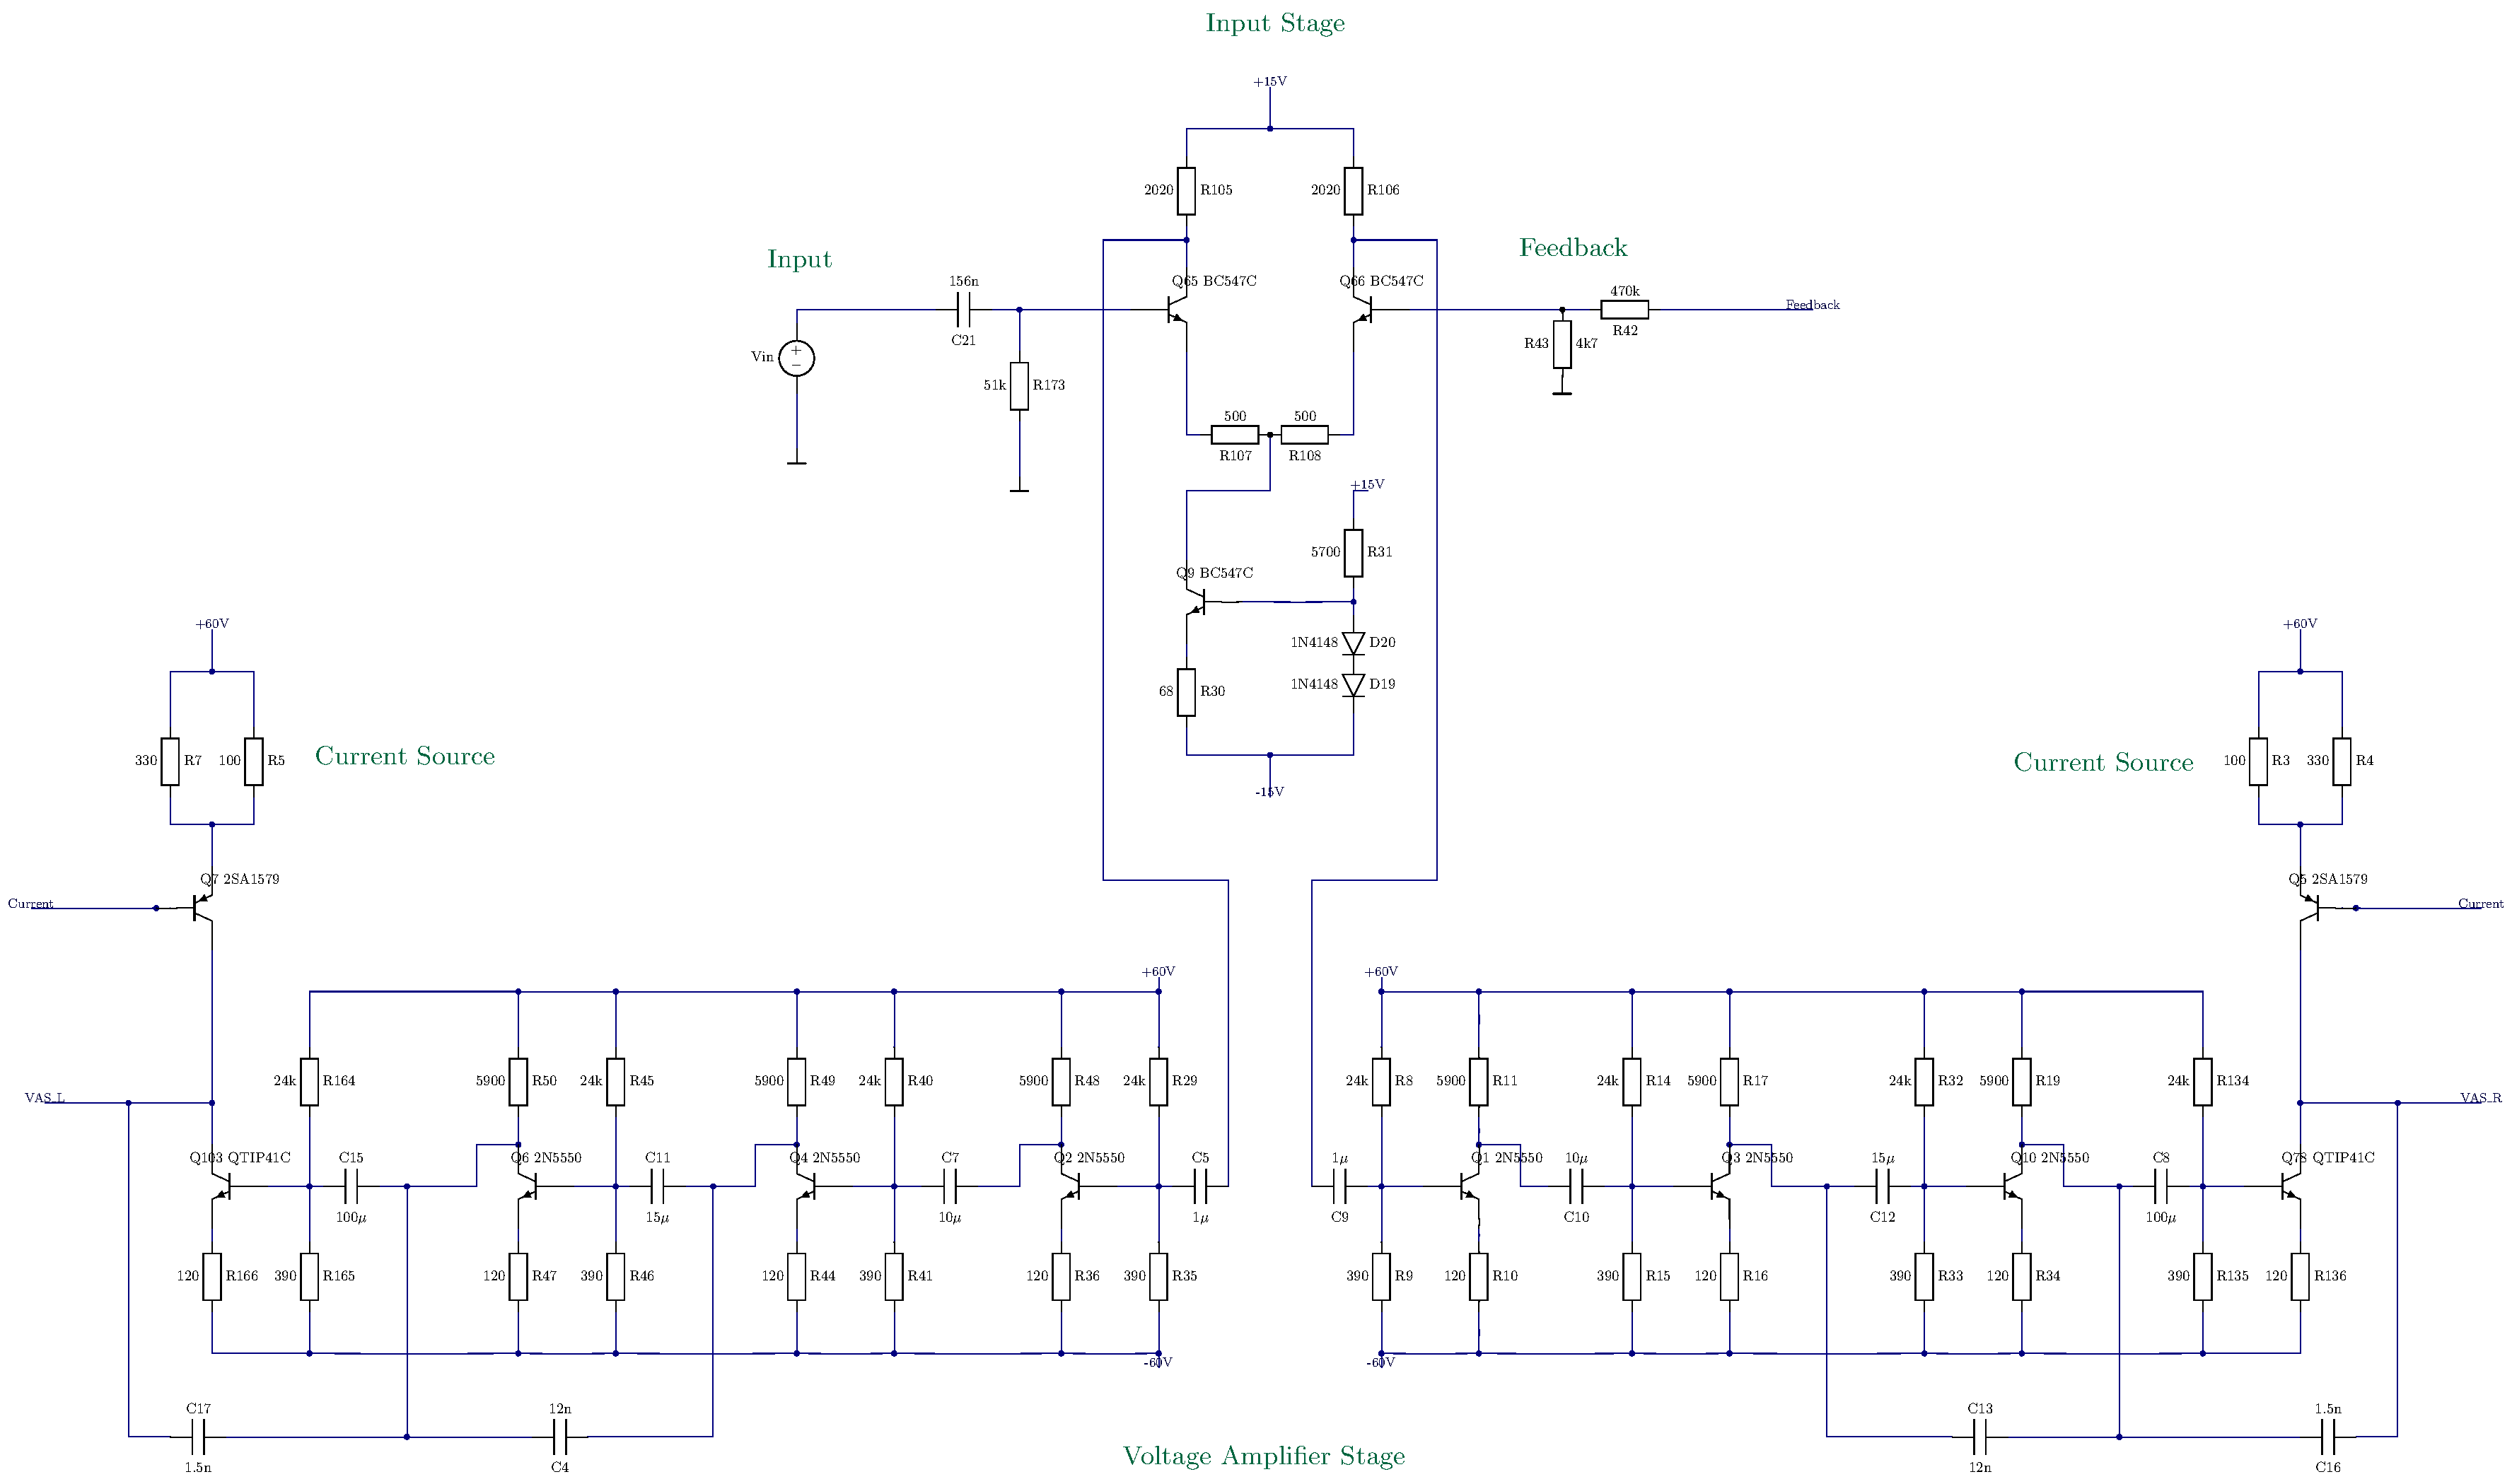
\includegraphics[width=\textwidth]{ImagenesCaracteristicas/TEX1.pdf}
	\caption{Etapas de entrada y amplificación. (Imagen vectorizada la cual no se pixelea)}
	\label{fig:circ}
\end{figure}
 \begin{figure}[H]
\centering
	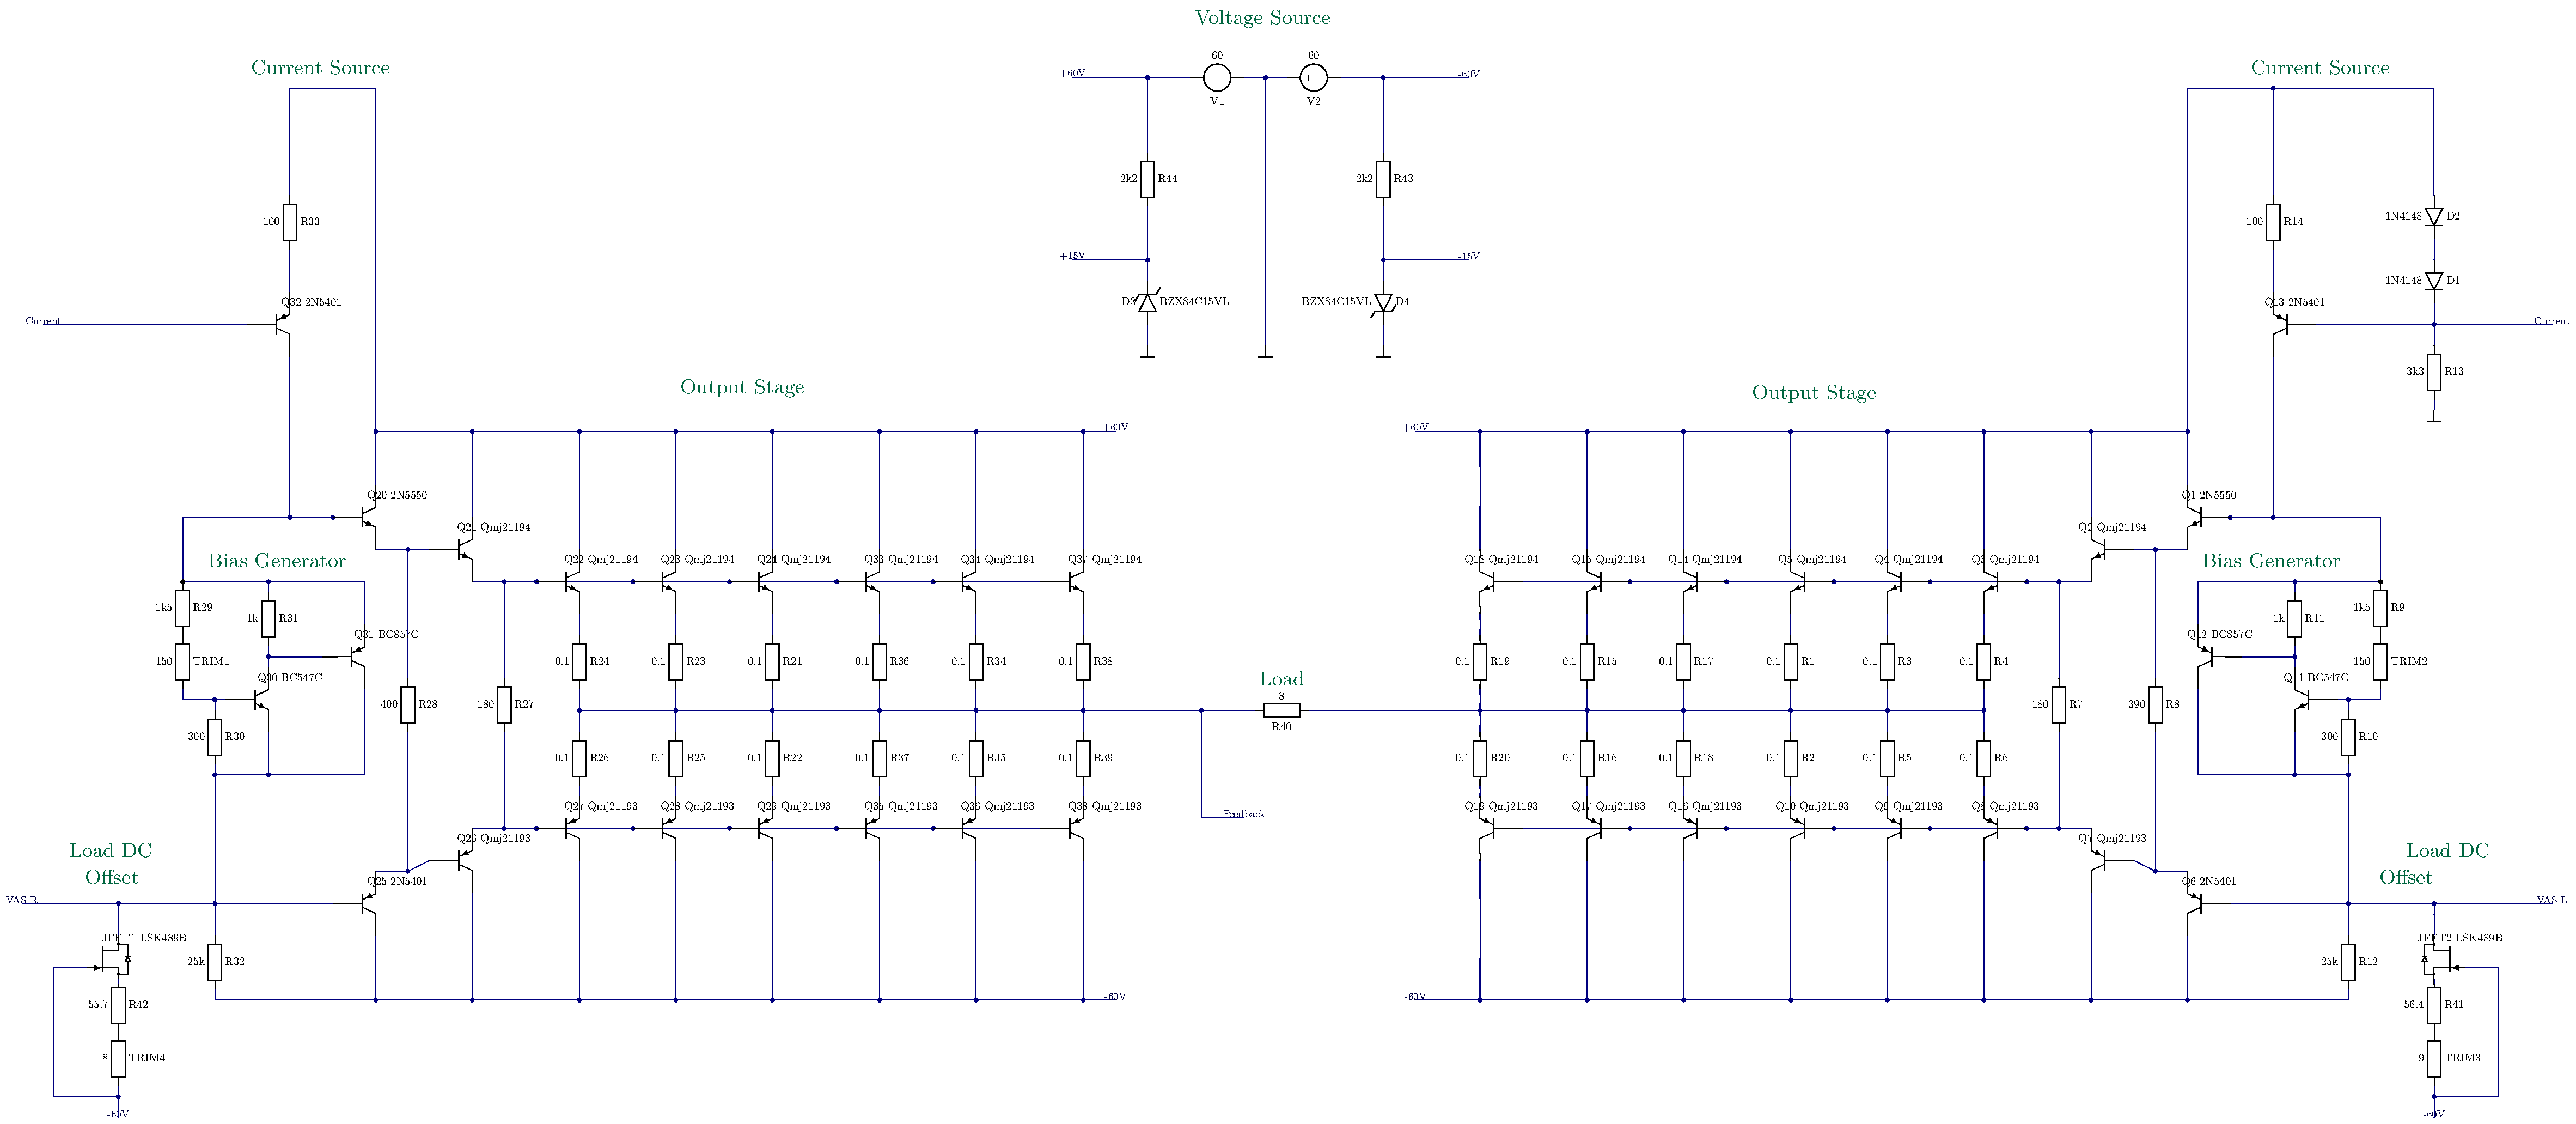
\includegraphics[width=\textwidth]{ImagenesCaracteristicas/TEX2.pdf}
	\caption{Etapas de salida y carga. (Imagen vectorizada la cual no se pixelea)}
	\label{fig:circ2}
\end{figure}

\begin{itemize}
\item Potencia máxima sin recorte sobre la carga de $1.5k \ W$.
\item Tensión pico sin recorte sobre la carga de $109 \ V$ con una fuente de alimentación de $\pm 60V$.
\item Dos etapas de salida clase AB en configuración puente H.
\item Rendimiento del amplificador del $74.5\%$ posterior al balanceo. (Ver últimos dos items)
\item Respuesta pasabanda en frecuencia para el rango audible con $-3 \ dB$ en $20-20k \ Hz$ respecto a la banda pasante.
\item El circuito se mantiene estable frente a ruido de distinta naturaleza y mantiene una salida sinusoidal.
\item Cuenta con una impedancia de entrada de $50 \ k\Omega$ en toda la banda audible.
\item Implementación con una única fuente partida.
\item Cuenta con una distorsión armónica del $\%$
\item El circuito cuenta con la posibilidad de ajustar el nivel de continua sobre la carga.
\item Permite calibrar el nivel de continua en reposo sobre los transistores de salida.

\end{itemize}

